\chapter{Schaltung}
Abbildung \ref{schaltung} zeigt den Schaltplan der Projekts. Auf der einen Seite ist der Raspberry PI erkennbar. Auf der anderen Seite befindet sich ein Arduino UNO, welcher einen Datenlogger darstellen soll. Da zur Zeit der Entwicklung der Datenlogger nicht vorhanden war, wurde mittels eines Arduino UNO dessen Funktionalitäten nachgebaut. Der Arduino UNO zählt die ankommenden Impulse und summiert diese auf. Per Konsole werden die Werte an den Entwickler gegeben, sodass er testen kann, ob die gewünschte Anzahl von Impulsen angekommen ist. Im Betrieb soll jedoch ein richtiger Datenlogger zum Einsatz kommen.\\
Der Kern des Schaltplans bildet der Optokoppler vom Typ KB Knighbright KB 817. Der Optokoppler trennt die beiden Stromkreise voneinander galvanisch. Diese Trennung sicheret den Raspberry PI gegen hohen Spannungen ab und verhindert somit seine Zerstörung. 
\begin{figure}[H]
 	\centering
 	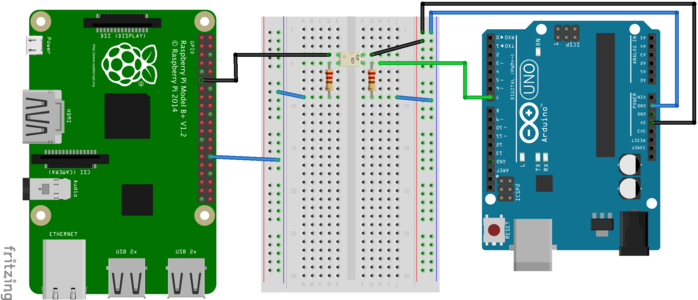
\includegraphics[width=0.8\textwidth]{bilder/schaltung.png}
 	\caption{Schaltung}
	\label{schaltung}
\end{figure}
